\documentclass[12pt, t]{beamer}
\usepackage{graphicx}
\usepackage{amsmath}
\usepackage{setspace}
\usepackage{float} 
\usepackage{multido}
\usepackage{multirow}
\usepackage{array}
\usepackage{enumerate}
\usepackage{booktabs}
\usepackage{indentfirst} 
\usepackage[style=mla]{biblatex}
\usepackage{subcaption}
\usepackage{hyperref}
\usepackage{textpos}
\usepackage{mathtools, nccmath}
\usepackage{ mathrsfs }

\makeatletter
\let\@@magyar@captionfix\relax
\makeatother

\definecolor{Turquoise3}{RGB}{0, 134, 139}
\renewcommand{\emph}[1]{{\color{Turquoise3}\textsl{#1}}}
\newcommand{\C}{\mathbb{C}} \newcommand{\F}{\mathbb{F}} \newcommand{\R}{\mathbb{R}} \newcommand{\Q}{\mathbb{Q}}
\newcommand{\N}{\mathbb{N}}
\newcommand{\myseries}[2]{$#1_1,#1_2,\dots,#1_#2$}
\newcommand{\nullspace}{~\\[15pt]}
\newcommand{\remark}{\textbf{Remark: }}
\newcommand{\scp}[2]{\langle\,#1\,,\,#2\,\rangle} \newcommand{\scpp}{\langle\,\cdot\,,\,\cdot\,\rangle}


\usetheme{Madrid}
\setbeamertemplate{navigation symbols}{}

\addtobeamertemplate{frametitle}{}{
\begin{textblock*}{100mm}(0.85\textwidth,-1cm)

\includegraphics[height=1cm]{Figures/logo/logo.png}
\end{textblock*}}

\definecolor{themecolor}{RGB}{25,25,112} 

\usecolortheme[named=themecolor]{structure}

\setbeamertemplate{items}[default]

\hypersetup{
    colorlinks=true,
    linkcolor=themecolor,
    filecolor=themecolor,      
    urlcolor=themecolor,
    citecolor=themecolor,
}

\title{VV186 Mid 2 Big RC}
\subtitle{\textbf{Differentiation of Real Functions and their Properties}\\``Sometimes you need to admit that, practice really makes perfect."}
\institute[UM-SJTU JI]{University of Michigan-Shanghai Jiao Tong University Joint Institute}
\author{Pingbang Hu}

\begin{document}

\begin{frame}
    \titlepage
    \begin{center}
        
\includegraphics[height=2cm]{Figures/logo/logo2.png}
    \end{center}
\end{frame}

\begin{frame}
    \frametitle{Overview}
    \begin{enumerate}
        \item Differentiation
        \item Derivative
        \item Rules of Differentiation
        \item Application of Differentiation
        \item Convexity and concavity
        \item L'Hopital's Rule
        \item Exercise
    \end{enumerate}
\end{frame}

\section{Differentiation}
\begin{frame}
    \frametitle{Differentiation}

In order to investigate a function's derivative, we should first take a close look of \textbf{Linear map}.

\vspace{2em}
\textbf{Definition : } A linear map on $\mathbb{R}$ is a function given by :
\begin{equation*}
    L: \mathbb{R}\rightarrow\mathbb{R}, \qquad L(x)=\alpha x, \alpha \in \mathbb{R}
\end{equation*}

\vspace{1em}
We would like to \emph{approximate} any functions which we are interested in by a linear map. And if 
such linear map exists, we say this function is \emph{differentiable}.
\end{frame}

\section{Differentiation}
\begin{frame}
    \frametitle{Differentiation}

\textbf{Definition : } 
    Let $\Omega\subseteq\mathbb{R}$ be a set and $x\in \text{int}\Omega$. Moreover, Let $f:\Omega\rightarrow \mathbb{R}$ be a real function. 
    Then we say $f$ is \textbf{differentiable} if there exists a linear map $L_x$ such that for all sufficiently small $h\in\mathbb{R}$, 
\begin{equation*}
    f(x+h)=f(x)+L_x(h)+o(h)\quad as\ h\rightarrow 0
\end{equation*}
This linear map is \textbf{unique}, if it exists. \\
\vspace{1em}
We call $L_x$ "the derivative of $f$ at $x$". If $f$ is differentiable at all points of some open 
set $U\subseteq \Omega$, we say $f$ is differentiable on $U$. 

\end{frame}

\section{Derivative}
\begin{frame}
    \frametitle{Derivative}

There is an important thing that you should pay attention to.\\ 

\vspace{0.5em}
\hspace{1em}
If you want to use the definition to calculate the derivative of some function $f$, you \textbf{need} to show how the extra terms belong to 
$o(h)$.\\

\vspace{1em}
\textbf{Exercise:}
\hspace{1em}
Use the definition to show 
\begin{equation*}
    \frac{d}{dx}\sin{x}=\cos{x}
\end{equation*}
(Hint: Consider how to take advantage of $o(h)$)
\end{frame}

\section{Derivative}
\begin{frame}
    \frametitle{Derivative}
Does the following statement make sense?

\vspace{0.5em}
    \begin{center}
        $L_x$ is a number for a fixed $x\in \Omega$, because $L_x=\alpha$.
    \end{center}
\vspace{0.5em}


\end{frame}


\section{Derivative}
\begin{frame}
    \frametitle{Derivative}
Does the following statement make sense?

\vspace{0.5em}
    \begin{center}
        $L_x$ is a number for a fixed $x\in \Omega$, because $L_x=\alpha$.
    \end{center}
\vspace{0.5em}
\hspace{1em}
$L_x$ is \textbf{not a number}, but a \textbf{linear map}, or one can say "linear function", so it essentially is a \emph{function}.
$L_x\cdot h=\alpha\cdot h$ (for some $\alpha$) doesn't mean $L_x=\alpha$.\\
\hspace{1em} To see this, one can consider a function given by 
\begin{equation*}
    f(x)=2x
\end{equation*}
,which doesn't mean $f=2$.\\

\end{frame}

\section{Derivative}
\begin{frame}
    \frametitle{Derivative}
Does the following statement make sense?

\vspace{0.5em}
    \begin{center}
        For $f(x)=x^4$, $f'(x)=4x^3$, so $L_x$ may not be linear
    \end{center}
\end{frame}


\section{Derivative}
\begin{frame}
    \frametitle{Derivative}
    Does the following statement make sense?

\vspace{0.5em}
    \begin{center}
        For $f(x)=x^4$, $f'(x)=4x^3$, so $L_x$ may not be linear
    \end{center}
\vspace{0.5em}

\hspace{1em} You are confusing "derivative at a point" with "function that gives derivative".
At certain point $x$, $4x^3$ is just a number in $\mathbb{R}$ (corresponds to the $\alpha$ for the definition of a linear map). 
Using our notation for $L_x$(or $f'(x))$, we can express $L_x$ as 
\begin{equation*}
    L_x(\cdot)=4x^3(\cdot)
\end{equation*}
, the \emph{variable} of $L_x$ is not $x$, so $L_x$ is \textbf{linear} for its input $(\cdot)$\\
\vspace{1em}
Given a differentiable function $f:\Omega\rightarrow\mathbb{R}$, the function 
that gives a derivative can be denoted by $L:\Omega\rightarrow\mathbb{R},\ L(x)=L_x(\cdot)$.\\
\textbf{It is a function that maps function to function}.
\end{frame}


\section{Derivative}
\begin{frame}
    \frametitle{Derivative}
\textbf{Exercise : }\\
\vspace{0.5em}
\hspace{1em}
What are the following objects really are?

\begin{enumerate}
    \item $\frac{d}{dx}$
    \vspace{1em}
    \item $\frac{d}{dx}f=f'$
    \vspace{1em}
    \item $f'(x)$
    \vspace{1em}
\end{enumerate}

Consider further, what are their domain and range?
\end{frame}

\section{Rules of Differentiation}
\begin{frame}
    \frametitle{Rules of Differentiation}
We not assume both $f$ and $g$ are differentiable functions, then:
\begin{itemize}
    \item $(f+g)'(x)=f'(x)+g'(x)$
    \vspace{1em}
    \item $(f\cdot g)'(x)=f'(x)g(x)+f(x)g'(x)$
    \vspace{1em}
    \item $(f\circ g)'(x)=f'(g(x))g'(x)$
    \vspace{1em}
    \item $(\frac{f}{g})'(x)=\frac{f'(xg(x)-f(x)g'(x))}{g^2(x)}$
    \vspace{1em}
    \item $f^{-1'}(y)=\frac{1}{f'(f^{-1}(y))}$
    \vspace{1em}
    \item $\underset{x\searrow b}{\lim}\frac{f(x)}{g(x)}=\underset{x\searrow b}{\lim}\frac{f'(x)}{g'(x)}$
    , if $\underset{x\searrow b}{\lim}\frac{f(x)}{g(x)}=\frac{0}{0}\text{ or }\frac{\infty}{\infty}$ and $\underset{x\searrow b}{\lim}\frac{f'(x)}{g'(x)}$ exists.
\end{itemize}
\end{frame}

\section{Application of Differentiation}
\begin{frame}
    \frametitle{Application of Differentiation}
We now list some Results and Theorems that you should already be familiar with.\\
\vspace{1em}
\begin{enumerate}
    \item If a real function is differentiable at $x$, then it is continuous at $x$.
    \vspace{0.5em}
    \item \emph{Hierarchy} of local smoothness.
    \begin{itemize}
        \item Arbitrary function
        \item Function continuous at $x$
        \item Function differentiable at $x$
        \item Function continuously differentiable at $x$
        \item Function twice differentiable at $x$
        \item \dots
    \end{itemize}
\end{enumerate}


\end{frame}

\section{Application of Differentiation}
\begin{frame}
    \frametitle{Application of Differentiation}
Result and Theorems.\\
\begin{enumerate}
    \item[3.] Let $f$ be a function and $(a,b)\subseteq \text{dom}\  f$ and open interval. If $x\in(a,b)$ is a 
        maximum(or minimum) point of $f\subseteq(a,b)$ and if $f$ is differentiable at $x$, then $f'(x)=0$.
    \vspace{0.5em}
    \item[4.] Let $f$ be a function and $[a,b]\subseteq \text{dom}\  f$. Assume that $f$ is differentiable on $(a,b)$ and 
        $f(a)=f(b)$. Then there is a number $x\in(a,b)$ such that $f'(x)=0$.\\
        \vspace{0.3em}
        Comment. We need the requirement that $f$ is \textbf{differentiable everywhere} on $(a,b)$. Otherwise, a 
        counterexample can be:
        \begin{equation*}
            [a,b]=[0,2],\quad 
            \begin{cases}
                f(x)=x\qquad &x\in[0,1]\\
                f(x)=2-x\quad &x\in(1,2]
            \end{cases}
        \end{equation*}
        
\end{enumerate}


\end{frame}

\section{Application of Differentiation}
\begin{frame}
    \frametitle{Application of Differentiation}
Result and Theorems.\\
\begin{enumerate}
    \item[5.] Let $[a,b]\subseteq\text{dom}\ f$ be a function that is continuous on $[a,b]$ and differentiable on $(a,b)$.
        Then there exists a number $x\in(a,b)$ such that $f'(x)=\frac{f(b)-f(a)}{b-a}$.
    \vspace{0.5em}
    \item[6.] Let $f$ be a real function and $x\in \text{dom}\ f$ such that $f'(x)=0$. If $f''(x)>0$, then $f$ has a local minimum at $x$, 
        if $f''(x)<0$, then $f$ has a local maximum at $x$.\\
    \vspace{0.3em}
    Comment. The case in which $f''(x)=0$ is more complicated, different conditions may occur.\\
    \hspace{1em}Example 1: $f'(x)=x^2$.    
    \hspace{1em}Example 2: $f'(x)=x^3$.\\
    As you can see from example 2, $f$ may not even have a local extremum if $f''(x)=0$.

\end{enumerate}


\end{frame}

\section{Application of Differentiation}
\begin{frame}
    \frametitle{Application of Differentiation}
Result and Theorems.\\
\begin{enumerate}
    \item[7.] Let $f$ be a twice differentiable function on an open set $\Omega\subseteq \mathbb{R}$. 
        If $f$ has a local minimum at some point $a\in \Omega$, then $f''(a)\geq 0$ .
\end{enumerate}
\textbf{Proof : }\\
\hspace{1em} Suppose $f$ has a local minimum at $a$. If $f''(a)<0$, then $f$ would also have a local maximum at $a$. 
Thus, $f$ would be constant in some interval containing $a$. So $f''(a)=0$. But this contradicts to our assumption.\\
\vspace{2em}
Comment. An analogous statement is : If $f$ has a local maximum at some point $a\in\Omega$, then $f''(a)\leq 0$.

\end{frame}

\section{Application of Differentiation}
\begin{frame}
    \frametitle{Application of Differentiation}
Result and Theorems.\\
\begin{enumerate}
    \item[8.] Let $a\in(0,\infty)\cup\{\infty\}$. Let $f:(-a,a)\rightarrow\mathbb{R}$ be a differentiable function. 
        If $f$ is odd, then its derivative is even; if $f$ is even, then its derivative is odd. 
\end{enumerate}

\textbf{Proof :}\\
\hspace{1em} Suppose $f$ is odd. Then
\begin{equation*}
    f'(-x)=\underset{h\rightarrow 0}{\lim}\frac{f(-x+h)-f(-x)}{h}=\underset{h\rightarrow 0}{\lim}\frac{f(x)-f(x-h)}{h}=f'(x)
\end{equation*} 
(Are there a more elegant way to proof it?)
\end{frame}


\section{Convexity and Concavity}
\begin{frame}
    \frametitle{Convexity and Concavity}

For further analysis of functions, we would introduce the concept of \textbf{Convexity} and \textbf{Concavity}. \\
The definition of these two concepts are as follows.\\

\hspace{1em}
Let $\Omega\subseteq\mathbb{R}$ be any set and $I\subseteq\Omega$ an interval. A function $f:\Omega\rightarrow\mathbb{R}$ 
is called convex on $I$ if for all 

\begin{equation*}
    x, a, b\in I \text{ with } a<x<b, \frac{f(x)-f(a)}{x-a}\leq\frac{f(b)-f(a)}{b-a}
\end{equation*}

\vspace{0.5em}
\hspace{1em}
A strictly convex function is a function that satisfies 
\begin{equation}
    \frac{f(x)-f(a)}{x-a}<\frac{f(b)-f(a)}{b-a}.
\end{equation}

\hspace{1em}
We say a function $f$ is concave if $-f$ is convex. We say a function $f$ is strictly concave if $-f$ is strictly convex.
\end{frame}

\section{Convexity and Concavity}
\begin{frame}
    \frametitle{Convexity and Concavity}
Comment. \\
\vspace{0.5em}
\hspace{1em}
We often use "$-$"(minus sign) to define a new definition from an existing one. The benefit is that these two definitions can 
be strongly related with each other.\\
\vspace{1em}
Comment 2.\\
\hspace{1em}
There is a quick way to memorize it\dots\hspace{2em}Con\textbf{cave}\dots
\begin{figure}[H]
    \centering
    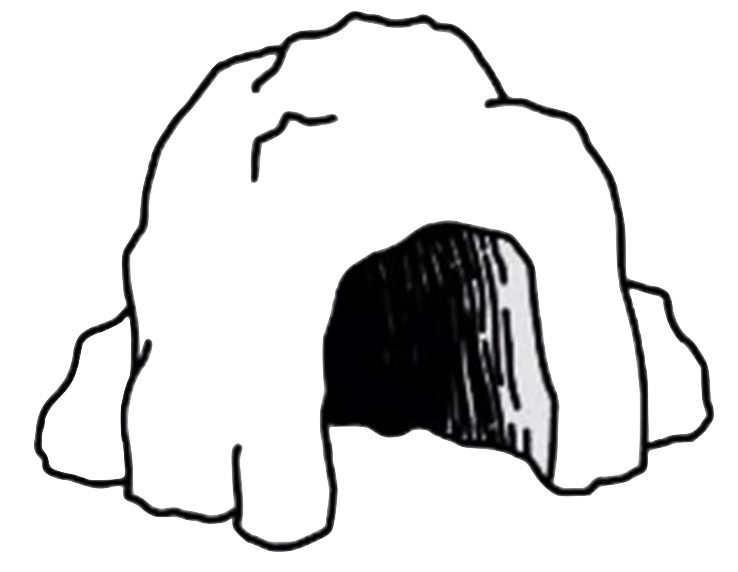
\includegraphics[width=5cm]{Figures/Concave.png}
\end{figure}
\end{frame}


\section{Convexity and Concavity}
\begin{frame}
    \frametitle{Convexity and Concavity}
As before, we list some Results and Theorems that you should already be familiar with.\\
\vspace{1em}

1. Let $f:I\rightarrow\mathbb{R}$ be strictly convex on $I$ and differentiable at $a,b\in I$. Then:
\begin{enumerate}
    \item[i] For any $h>0(h<0)$ such that $a+h\in I$, the graph of $f$ over the interval $(a,a+h)$ lies below the secant line through the 
        points $(a,f(a))$ and $(a+h, f(a+h))$
    \item[ii] The graph of $f$ over all $I$ lies above the tangent line through the point $(a, f(a))$
    \item[iii] If $a<b$, then $f'(a)<f'(b)$
\end{enumerate}
\end{frame}

\section{Convexity and Concavity}
\begin{frame}
    \frametitle{Convexity and Concavity}
Results/Theorem \& Comment\\
\vspace{1em}
2. A function $f:I\rightarrow\mathbb{R}$($I$ is an interval) is convex if and only if 
\begin{equation*}
    \underset{t\in(0,1)}{\forall}\ \underset{x,y\in I}{\forall}\text{ with } x<y, f(tx+(1-t)y)\leq tf(x)+(1-t)f(y)
\end{equation*}\\

\vspace{2em}

3. Let $I$ be an interval, $f:I\rightarrow\mathbb{R}$ differentiable and $f'$ strictly increasing. If $a, b\in I$, $a<b$ and 
$f(a)=f(b)$, then 
\begin{equation*}
    f(x)<f(a)=f(b)\text{ for all }x\in(a,b)
\end{equation*}

\end{frame}

\section{L'Hopital's Rule}
\begin{frame}
    \frametitle{L'Hopital's Rule}
When calculating the limit for some function, you may bump into some cases including:
\begin{center}
    \begin{enumerate}
        \center \item[i] $\underset{x\rightarrow a}{\lim}\ \frac{f(x)}{g(x)} =\frac{\infty}{\infty}$
        \center \item[ii]$\underset{x\rightarrow a}{\lim}\ \frac{(f(x)}{g(x)} = \frac{0}{0}$ 
    \end{enumerate}
\end{center}

\hspace{1em}
in both cases, the right-hand side is the \emph{pre-result} when you are trying to plug in the limit point into your function 
(in this case, $\frac{f(a)}{g(a)}$) 
and guess the result. \\

\hspace{1em}
However, you might encounter above cases and then you have no idea what the limit is. \\
\hspace{1em}
Fortunately, we have L'Hopital's Rule.


\end{frame}

\section{L'Hopital's Rule}
\begin{frame}
    \frametitle{L'Hopital's Rule}
Here is the theorem.\\
\hspace{1em}
Let $f$ and $g$ be real functions such that the $b\in\overline{domf\cap domg}$ and 
$\underset{x\searrow b}{\lim}f(x)=\underset{x\searrow b}{\lim}g(x)=0$. Suppose further that $f$ and $g$ are defined and differentiable on 
$(b,b+\delta)$ and $g'(x)\neq 0$ on it. Moreover, if the limit $\underset{x\searrow b}{\lim}\ \frac{f'(x)}{g'(x)}=:L$ exists, then 
\begin{equation*}
    \underset{x\searrow b}{\lim}\ \frac{f(x)}{g(x)}=\underset{x\searrow b}{\lim}\ \frac{f'(x)}{g'(x)}=L
\end{equation*}
Comments. This result doesn't require dealing with whole neighborhood, but instead, \emph{half-neighborhood}.\\
\vspace{0.5em}
\hspace{1em} 
As $b\rightarrow \infty$, we expect a similar method will hold, which is shown in next slide.
\end{frame}

\section{L'Hopital's Rule}
\begin{frame}
    \frametitle{L'Hopital's Rule}
Let $f$ and $g$ be real functions such that the interval $(C,\infty)\subseteq domf\cap domg$ and 
$\underset{x\rightarrow \infty }{\lim}f(x)=\underset{x\rightarrow \infty }{\lim}g(x)=0$. Suppose further that $f$ and $g$ are defined 
and differentiable on $(C,\infty)$ and $g'(x)\neq 0$ on it. Moreover, if the limit $\underset{x\rightarrow \infty }{\lim}\ \frac{f'(x)}{g'(x)}=:L$ exists, then 
\begin{equation*}
    \underset{x\rightarrow\infty}{\lim}\ \frac{f(x)}{g(x)}=\underset{x\rightarrow\infty}{\lim}\ \frac{f'(x)}{g'(x)}=L
\end{equation*}
    
\vspace{0.5em}
\hspace{1em}
Actually, we have one more variations of L'Hopital's Rule.
\end{frame}

\section{L'Hopital's Rule}
\begin{frame}
    \frametitle{L'Hopital's Rule}
Let $f$ and $g$ be real functions such that the interval $(C,\infty)\subseteq domf\cap domg$ and 
$\underset{x\rightarrow \infty }{\lim}f(x)=\underset{x\rightarrow \infty }{\lim}g(x)=\infty$. Suppose further that $f$ and $g$ are defined 
and differentiable on $(C,\infty)$ and $g'(x)\neq 0$ on it. Moreover, if the limit $\underset{x\rightarrow \infty }{\lim}\ \frac{f'(x)}{g'(x)}=:L$ exists, then 
\begin{equation*}
    \underset{x\rightarrow\infty}{\lim}\ \frac{f(x)}{g(x)}=\underset{x\rightarrow\infty}{\lim}\ \frac{f'(x)}{g'(x)}=L
\end{equation*}

\vspace{0.5em}
\hspace{1em}
The only difference is that $\underset{x\rightarrow\infty}{\lim}f(x)=\underset{x\rightarrow \infty }{\lim}g(x)=\infty$.    
\end{frame}


\section{Brief summary}
\begin{frame}
    \frametitle{Brief Summary}
    There are something you should know for this section.
    \vspace{1em}
\begin{enumerate}
    \item Be familiar with the definition of $L_x$
    \vspace{0.5em}
    \item Know the difference between $\frac{d}{dx}, \frac{df}{dx},f'(x)$, or further, $\frac{d^2}{dx^2}$ and so on\dots
    \vspace{0.5em}
    \item Get familiar with the basic calculation process for calculating a function's derivative.
    \vspace{0.5em}
    \item Know what are \textbf{Rolle's theorem}, \textbf{Mean Value theorem}, and also \textbf{Cauchy Mean Value Theorem}.
    \vspace{0.5em}
    \item Know when you can apply \textbf{L'Hopital's Rule} when you perform limit calculations.
\end{enumerate}
\end{frame}


\section{Exercise}
\begin{frame}
    \frametitle{Exercise}
1. Please calculate following functions' derivative.\\(Suppose $g'$ always exists and doesn't vanish)
\begin{enumerate}
    \item[i.]   $f(x)=g(x/g(a))$
    \item[ii.]  $f(x)=g(x+g(x))+{g(x+a)}$ 
    \item[iii.] $f(x) =ax\cdot g(x)$
    \item[iv.]  What is wrong with the following usage of L'Hopital's Rule?\\
        \begin{equation*}
            \underset{x\rightarrow 1}{\lim}\ \frac{x^3-x-2}{x^2-3x+2}=\underset{x\rightarrow 1}{\lim}\ \frac{3x^2-1}{2x-3}=\underset{x\rightarrow 1}{\lim}\ \frac{6x}{2}=3
        \end{equation*}
\end{enumerate}
\end{frame}


\section{Exercise}
\begin{frame}
    \frametitle{Exercise}
2. Prove that if 
\begin{equation*}
    \frac{a_0}{1}+\frac{a_1}{2}+\dots+\frac{a_n}{n+1}=0
\end{equation*}
Then $a_0+a_1x+\dots+a_nx^n=0$ for some $x\in[0,1]$
\end{frame}


\section{Exercise}
\begin{frame}
    \frametitle{Exercise}
3. Practical calculation shouldn't be ignored. Please calculate the derivatives of the following functions.
\begin{itemize}
    \item $(2x+5x^2)^6$
    \vspace{0.3em}
    \item $\frac{\sqrt{x}}{x+1}$
    \vspace{0.3em}
    \item $\sqrt[3]{\frac{3x^2+1}{x^2+1}}$
    \vspace{0.3em}
    \item $x^{x}$
\end{itemize}
    
\end{frame}

\section{Exercise}
\begin{frame}
    \frametitle{Exercise}
4. Remember the problem that asks you to calculate
\begin{equation*}
    \underset{x\rightarrow 1}{\lim}\frac{\sqrt{x+3}-\sqrt{3x+1}}{x-1}\ ?
\end{equation*} 
Now please use L'Hopital's rule to solve it. 
\end{frame}

\section{Exercise}
\begin{frame}
    \frametitle{Exercise}
5. Let $f$ be a continuous convex real function on $[a,b]$. Show that $f$ either has one local minimum or infinitely many local minimums on $[a,b]$.
\end{frame}


\section{Exercise*}
\begin{frame}
    \frametitle{Exercise*}
6. Suppose $f:[0,n],n\in \mathbb{N}$ is a continuous function, and is differentiable on $(0,n)$. Furthermore, assume that 
\begin{equation*}
    f(0)+f(1)+\dots+f(n-1)=n,\ f(n)=1
\end{equation*} 
Show that there must exist $c\in (0,n)$ such that $f'(c)=0$.

\end{frame}


\section{Exercise*}
\begin{frame}
    \frametitle{Exercise*}
7. Let $f,g$ be two differentiable functions with domain $[0,\infty)$.\\
Prove that if
\begin{equation*}
    f(0)=g(0)\ \text{and} \ f'(x)\geq g'(x)\ \text{for all }x>0
\end{equation*}
then 
\begin{equation*}
    f(x)\geq g(x) \text{ on } [0,\infty)
\end{equation*}
\end{frame}

\section{Exercise*}
\begin{frame}
    \frametitle{Exercise*}
8. Suppose that $f$ satisfies $f''+f'g-f=0$ for some function $g$. Prove that if $f$ is 0 at two distinct points, 
then $f$ is 0 on the interval between them.
\end{frame}


\begin{frame}
    \frametitle{End}
    \vspace{2cm}
    \Huge \center  Have Fun and Learn Well!
\end{frame}
\end{document}